\chapter{Il petrolio}
\section{Cosa � il petrolio?}
La definizione merceologica italiana di \textit{petrolio} lo indica come materiale combustibile liquido, oleoso, pi� o meno viscoso, di colore da bruno chiaro a nero, di odore spesso sgradevole, che si incontra in natura in rocce sedimentarie.

Nell'accezione anglosassone, invece petrolio (petroleum), � inteso come miscela complessa di idrocarburi reperibile in natura. Essa pu� trovarsi nelle forme solida, liquida o gassosa prendendo in tali casi rispettivamente il nome di \textit{asfalto} (asphalt), \textit{greggio} (crude oil) o \textit{gas naturale} (natural gas).

D'ora in poi indicheremo con il termine di \textit{petrolio} ci� che nella definizione anglosassone � indicato da \textit{crude oil}, ovvero una miscela di idrocarburi reperibile in natura allo stato liquido.

A partire dal 1960 il petrolio rappresenta la maggior fonte energetica mondiale.

\section{Composizione}

All'interno della miscela definita come petrolio possono essere trovati molti idrocarburi, a loro volta classificabili in diverse categorie.

Gli idrocarburi, alle condizioni di pressioni e temperatura ambiente, si possono ritenere gassosi se di dimensioni ridotte (\ce{C_1}-\ce{C_4}), liquidi (da \ce{C_5} a \ce{C_{17}}) e solidi (se puri) quelli di dimensioni superiori.

Una ulteriore classificazione pu� essere effettuata analizzando le \textit{strutture molecolari}, infatti si hanno idrocarburi lineari, ramificati e ciclici. La presenza di \textit{insaturazioni} (doppi legami) inseriscono una ulteriore suddivisione, classificandole in \textit{paraffine} (senza doppi legami), \textit{olefine} (con doppi legami ma non strutture aromatiche) e \textit{aromatici} (doppi legami in strutture aromatiche).

La composizione del petrolio, come evidente dal diagramma di \textit{Francis} (\figurename~\ref{fig:Pet:DiagFrancis}) � costituita esclusivamente da paraffine e aromatici, poich� per le olefine si avrebbe la decomposizione ai loro elementi costitutivi ($C$ e $H_2$), essendo il loro $\Delta G^o$ maggiore di 0 a ogni temperatura. Inoltre, pur essendo un processo cineticamente lento, hanno avuto a loro disposizione migliaia di anni per decomporsi.
\begin{figure}[htbp]
	\centering
		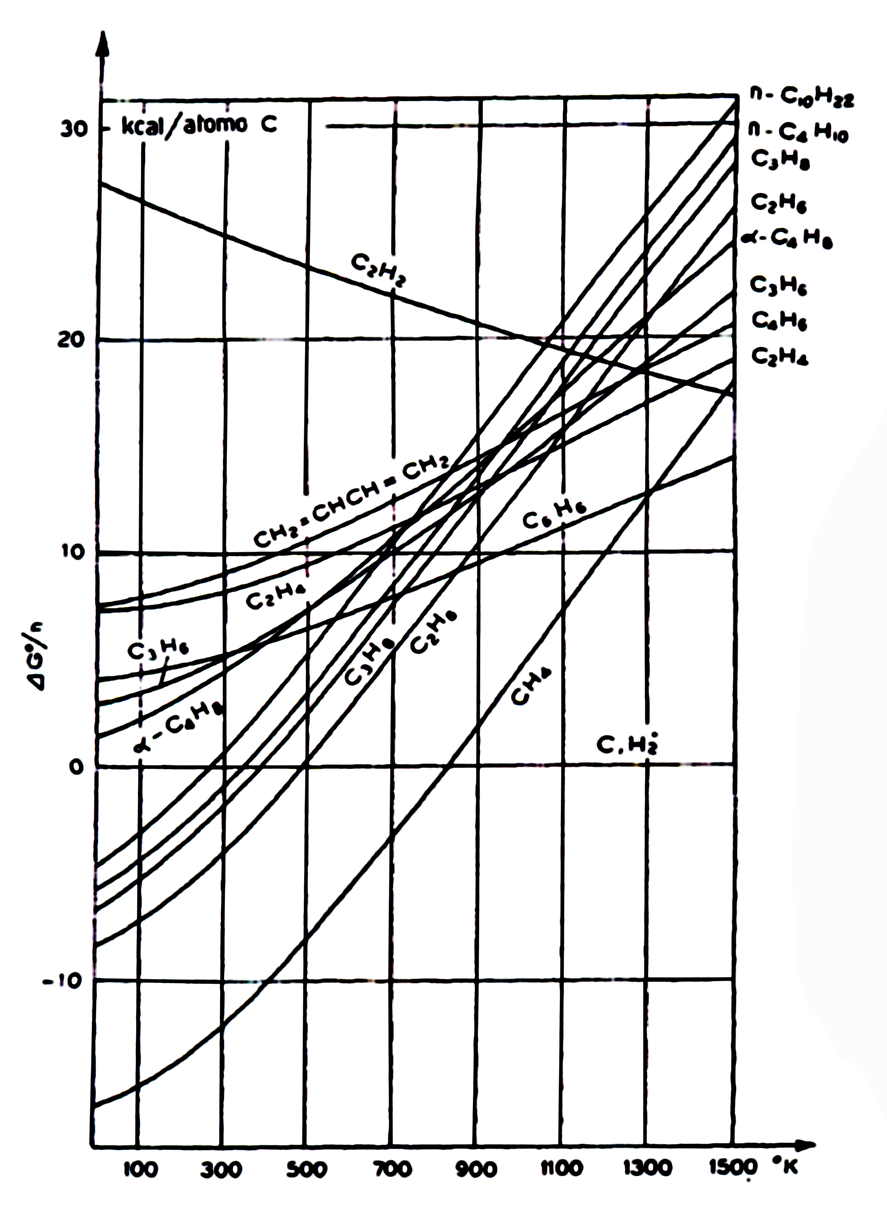
\includegraphics[width=0.90\textwidth]{image/PetDiagFrancis.png}
	\caption{Diagramma di \textit{Francis} per gli idrocarburi.}
	\label{fig:Pet:DiagFrancis}
\end{figure}

\section{Prodotti}
I prodotti derivati dal petrolio sono costituiti all'80-90\% da combustibili e carburanti. I prodotti utilizzati come combustibili sono suddivisi a loro volta in combustibili gassosi quali gas di raffineria ($CH_4$, $C_2H_6$), GPL ($C_3H_8$, $C_4H_{10}$) e combustibili liquidi. Questi si suddividono a loro volta in funzione della temperatura di ebollizione in:
\begin{itemize}
	\item benzine per autotrazione ($T_{eb} = 40-200^oC$)
	\item kerosene ($T_{eb} = 175-225^oC$)
	\item gasolio ($T_{eb} = 200-400^oC$)
	\item oli pesanti combustibili ($T_{eb} > 350^oC$)
\end{itemize}
I prodotti non utilizzato come combustibili, invece, sono:
\begin{itemize}
  \item GPL e nafta, usati nell'industria petrolchimica
  \item paraffine, usate nelle industrie chimiche, della carta e in medicina
  \item distillati pesanti, usati nella produzione di lubrificanti e grassi
  \item residui pesanti per la produzione di bitumi e asfalti 
  \item coke da petrolio, usato per la produzione di elettrodi
\end{itemize}

\subsection{I vantaggi nell'uso del petrolio}
L'uso del petrolio come materia prima per l'industria chimica � stato favorito da diversi fattori, innanzi tutto il rapporto tra l'idrogeno e il carbonio presente nella miscela di partenza ($H/C \approx 2$) � abbastanza vicino al valore presente nella maggior parte di composti di partenza dell'industria chimica organica (soprattutto per quanto riguarda monomeri e polimeri plastici). Altro fattore che ha influenzato la sua diffusione � la facilit� di trasposto dalle zone produttive alle zone di lavorazione, inoltre il suo commercio � regolamentato a livello mondiale. Come sar� evidente pi� avanti gli stessi processi utilizzati per incrementare la frazione leggere per usi energetici portano anche alla formazione dei principali intermedi di base dell'industria chimica organica (etilene, propilene, \ce{C_4}, BTX, ...); infine anche \ce{NH_3} e \ce{SO_3}, capostipiti della chimica industriale inorganica, derivano, almeno in parte, da cicli di raffineria.

\section{Trattamenti iniziali}
\subsection{Dissalazione}
Il petrolio in arrivo alla raffineria deve essere inizialmente trattato per estrarre i sali presenti, infatti il petrolio, essendo stato estratto dal sottosuolo, contiene in emulsione dei sali che possono provocare processi di corrosione sulle successive apparecchiature dell'impianto. Il processo di dissalazione pu� seguire diverse vie:
\begin{itemize}
	\item si procede ad un lavaggio con acqua per estrarre i sali;
	\item si sottopone il grezzo ad una separazione elettrostatica, facendogli attraversare una zona ad alta differenza di potenziale;
	\item facendo percolare il greggio attraverso fibre e granuli che sottraggono i sali presenti;
\end{itemize}

\subsection{Topping}
A seguito di questa prima fase, si prosegue con una prima distillazione in una colonna a pressione atmosferica per la separazione delle principali classi di prodotti. Questo procedimento viene chiamato \textit{topping} in cui il petrolio iniziale attraversa due fasi differenti, si ha inizialmente una distillazione flash e una seconda fase di rettifica. Lo schema dell'impianto di topping � dato da uno scambiatore di calore dove si fa giungere il grezzo ad una pressione di circa 20Atm in cui si ha un preriscaldamento a scapito del calore fornito dai prodotti di distillazione. In seguito si trova un forno a tubi, dove si bruciano i prodotti di scarto del topping, e in cui la temperatura del petrolio viene portata a $340-360^oC$. All'uscita del forno il materiale di partenza viene inviato ad una camera di flash ($1.5 - 2Atm$) dove viene pi� o meno vaporizzato in funzione della sua composizione. Dopo l'espansione il greggio viene inviato ad una colonna di distillazione dove vengono separati i principali tagli (vedi \tablename~\ref{tab:Pet:TagliTopping}), i primi due (gas incondensabili e benzine leggiere) escono dalla testa della colonna sottoforma di vapore, la frazione di gasolio pesante esce dal fondo della colonna, mentre le frazioni intermedie vengono prelevate da posizioni diverse della colonna.
\begin{table}[htbp]
	\centering
		\begin{tabular}{lcc} \hline
			Frazione						& $T_{eb}^{inf}$ & $T_{eb}^{sup}$ \\ \hline
			Gas incondensabili	&								 & 							 	\\
			Benzine leggere			& 120 					 & 150 					 	\\
			Benzine pesanti			&	150 					 & 200 					 	\\
			Kerosene						& 175 					 & 225					  \\
			Gasolio leggero			& 250 					 & 320 					 	\\
			Gasolio pesante			&	360 					 & 							 	\\ \hline
		\end{tabular}
	\caption{Tagli petroliferi in uscita dal processo di \textit{topping}.}
	\label{tab:Pet:TagliTopping}
\end{table}

\subsection{Vacuum}
I prodotti in uscita dalla coda della colonna di topping non possono essere utilizzati tal quali, poich� contengono ancora una miscela di sostanze che devono essere separate, ma a causa della elevata temperatura di ebollizione ($360^oC$) che se ulteriormente aumentata porterebbe a disastrosi effetti di pirolisi, non � possibile operare una semplice rettifica a pressione atmosferica. 

Per evitare di dover operare a temperature elevate si ricorre ad una seconda colonna di distillazione che opera in depressione (il \textit{vacuum}, per cui la pressione operativa si aggira all'intorno dei $10-50mmHg$. L'abbassamento della pressione fa si che la temperatura di ebollizione sia inferiore e ci� consente di evitare i fenomeni di pirolisi. La depressione � realizzata ricorrendo ad una serie di eiettori a vapore disposti in serie e collegati alla testa della colonna.

In ingresso si hanno tutte le sostanze presenti sul fondo della colonna di topping, quindi cicloalcani, idrocarburi aromatici ad alto peso molecolare ed asfalteni, oltre ai residui carboniosi presenti. Dalla testa del vacuum si estrarranno gasoli pesanti, mentre le frazioni intermedie sono composte da oli combustibili. Dal fondo si estraggono bitumi utilizzati per la produzione di asfalto.